\renewcommand{\caseUseShortName}{buscarAvanzadoOrdenesProduccion} %cammelCase name

\renewcommand{\caseUseCreated}{05/03/2020} %Fecha creación
\renewcommand{\caseUseModified}{05/03/2020} %Fecha modificación
\renewcommand{\caseUseName}{\CUbuscarAvanzadoOrdenesProduccion- Buscar avanzado órdenes de producción} %{\CUcammelCase - Title}

\renewcommand{\caseUseSummary}{Este caso de uso permite a un fabricante de ZMGestion buscar órdenes de producción a partir de un producto, tela, lustre y estado.} %Resumen
\renewcommand{\caseUsePeople}{Fabricantes: quiere encontrar una orden de producción existente en el sistema.} %Actor: Meta
\renewcommand{\caseUsePreconditions}{
	\caseUseRow{Haber iniciado sesión en el sistema y tener el permiso necesario para realizar esta función.} %Precondiciones
}
\renewcommand{\caseUsePostconditions}{
	\caseUseRow{Ninguna.} %Postcondiciones
}
\renewcommand{\caseUseScene}{ %Escenario principal
    \addCaseUseStep{El fabricante accede a la pantalla para realizar la búsqueda de órdenes de producción.}
    \addCaseUseStep{ZMGestion muestra un formulario para que el fabricante seleccione un producto, tela, lustre y estado de la orden de producción. Siendo opcionales todos los campos solicitados.}
    \addCaseUseStep{El fabricante completa los campos solicitados.}
    \addCaseUseStep{ZMGestion realiza la búsqueda por producto, tela, lustre y estado de la orden de producción.}
    \addCaseUseStep{ZMGestion lista las coincidencias encontradas.}
}
\renewcommand{\alternativeCaseUse}{ %Flujos alternativos
	\newAlternative{A1: No se encontró ninguna coincidencia.}{4} %Flujo alternativo A1.
	\caseUseRow{La secuencia A1 comienza luego del punto 3 del escenario principal.} %¡Indicar número paso!
    \alternativeRow{ZMGestion informa al usuario que no se encontron resultados para su búsqueda.}
    \caseUseRow{El escenario vuelve al punto 2.}
}
%\item Caso de uso \caseUseName
\renewcommand*{\arraystretch}{1.3}
\begin{longtable}[c]{|>{\raggedright}p{0.3\textwidth} | >{\raggedright}p{0.2\textwidth} | p{0.5\textwidth} |}
\caption{\hyperref[sec:listadoCasoUso]{\caseUseName}}
\label{tabla:\caseUseShortName}\\
\hline
\rowcolor{tableCaseUseBackground}

\multicolumn{3}{|l|}{\textcolor{tableCaseUseFontColor}{Descripción textual del caso de uso: \caseUseName}} \\ \hline

Fecha de Creación: & \multicolumn{2}{L{\secondColumnWidth}|}{\caseUseCreated}\\ \hline

Fecha de Modificación: & \multicolumn{2}{L{\secondColumnWidth}|}{\caseUseModified} \\ \hline

Versión: & \multicolumn{2}{L{\secondColumnWidth}|}{1} \\ \hline

Resumen: & \multicolumn{2}{L{\secondColumnWidth}|}{\caseUseSummary} \\ \hline

Personas involucradas y metas: & \multicolumn{2}{L{\secondColumnWidth}|}{\caseUsePeople} \\ \hline

Precondiciones: \caseUsePreconditions \hline

Postcondiciones: \caseUsePostconditions \hline

Escenario principal: \caseUseScene \hline

Flujos alternativos: \alternativeCaseUse \hline

Requisitos de interfaz de usuario: \caseUseRequirementsGUI \hline
\multirow{3}{*}{Requisitos funcionales:}  & Tiempo de respuesta: & \caseUseResponseTime \\ \cline{2-3} 
& Concurrencia: & \caseUseConcurrence \\ \cline{2-3} 
& Disponibilidad: & \caseUseAvailability \\ \hline
\end{longtable}

\setcounter{rownumbers}{0}

\renewcommand{\alternativeCaseUse}{
	\caseUseRow{No existen flujos alternativos.}
}

%DIAGRAMA DE ACTIVIDAD
%\lineabreak[0]
\begin{figure}[H]
    \centering
    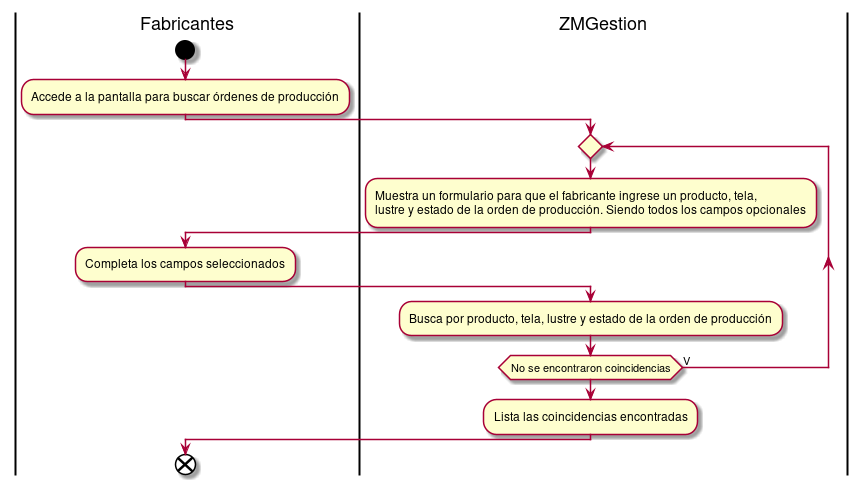
\includegraphics[width=\textwidth,height=0.95\textheight,keepaspectratio]{DiagramasActividad/DiagramaDeActividad/buscarAvanzadoOrdenesProduccion}
    \caption{CU92 - Buscar avanzado órdenes de producción}
\label{fig:buscarAvanzadoOrdenesProduccion}
\end{figure}